\section*{Results}


\subsection{The data}

The models were trained and tested on different points of 324 different pandemics generated with Covasim \cite*{kerr2021covasim}, a complex agent-based model. 
To generate those pandemics, four parameters that maximized the diversity of the set of pandemics generated were selected (see \ref{sec:generating_divserse_pandemics}). 
Those parameters were varied on the three values 0.5, 1 and 2. 
These values correspond to scaling factors of the default values of the model. 
For each pandemic, the transmission probabilities were time dependant and followed one of the four different mobility patterns (see \ref{fig:mobilities}). 
Thanks to those 4 parameters, each varied on three different values and to the four different mobilities, we obtained 324 simulations of pandemics. 
We decided to focus on the number of hospitalized individuals as the target variable. 
Indeed, it is a key variable to monitor, as the hospital occupancy correspond to the capacity of the state to treat the patients. 


\subsection*{The models}

In this paper, we implemented 13 individual models and an ensemble model.
Each model was trained on the data from the beggining of a pandemic and made predictions 7 or 14 days ahead (on user's choice).
They output a point prediction and a set of confidence intervals on the prediction. 
Models of two types were implemented. 
The first type models were only trained on the time-serie of the number of hospitalized of the past few days. 
The second type of models xere trained on the time series of the number of hospitalized, but also on the mobility data and the number of infected. 

\subsubsection{SIRH}

The SIRH (Suspectible, Infected, Recovered, Hospitalized) (\ref{fig:sirh}) is a variation of the classical SIR model, with another compartment : the Hopsitalized compartment. 
The parameters of this model correspond to the rates of evolution from a compartment to another one. 
$\beta$ correspond to the transmission rate, $\gamma_i$ and $\gamma_h$ correspond to the recovery rate from both Infected and Hospitalized compartments, and $h$ correspond to the hospitalization rate. 
The value of $S, I, R$ and $H$ are linked through a system of differential equations (\ref{eq:sirh}). 
As the curve of the pandemic of a SIRH is deterministic, it is possible to generate it from the values of the parameters $\beta$, $\gamma_i$, $\gamma_h$ and $h$, and to compare it to the value of the number of hospitalized observed from the beginning of the pandemic.
The optimal parameters are found through minimization of the least square between the SIRH curve and the real curve. 
During the predicting phase, a 7 (or 14) days SIRH is run, with initial value estimated from the data and the fit of the training phase.
The confidence interval is estimated through linearization of the regression (see \ref{sec:ci})

Variations of the SIRH model were implemented, with $\gamma_i$ and $\gamma_h$ kept constant. 

A SIRH model of the second type was also constructed. 
Following the same idea as the first type SIRH, this model has a time varying transmission rate, which is a linear combination of the mobility : $\beta_t = a \times m_t + b$. 
The parameters to optimize are now $a, b, \gamma_i, \gamma_h$ and $h$ and both curve of the number of hospitalized and the number of infected are fitted to the data. 


\subsubsection{ARIMA}

The ARIMA is a model used for time series forcasting. 
It is the sum of an AR and a MA model (\ref{eq:arima})
It is trained by maximizing the likelihood of the observed data. 

A VAR model, which is a multi-dimensional AR model was also implemented. 
It is also optimized through maximum likelihood. 

\subsubsection{Moving Average}

The moving average model is a baseline model that is used as a reference. 
It returns the value of the average of the past seven days and a confidence interval based on the variance of the values of the past seven days. 


\subsubsection{Exponential regression}

The exponential regression is a model that fits an exponential regression ($x \rightarrow a e^{b x} + c$ ) to the values of the number of hospitaized. 
The values of $a, b$ and $c$ are found by minimizing the least square difference between the prediction and the real values. 
The confidence interval is estimated through linearization of the regression (see \ref{sec:ci}). 

An exponential regression of the second type was also implemented. 
The number of hospitalized is then an exponential regression of both mobility data, number of infected and number of hospitalized shifted. 


\subsubsection{Regressors}

A Bayesian and a linear regressor were implemented.
They use the last 20 data points to predict the next one (see \ref{sec:mlmodels}). 


\subsection*{Evaluation of the models}

The models described above were tested on 14 points of each of the 324 pandemics generated. 
For each point, a 7 and 14 days-ahead prediction was made. 
Each prediction was evaluated thanks to WIS and RMSE (see \ref{sec:metrics}), and then ranked according to the performances of other models.
The point of evaluation were also classified in one of the following categories : 'big increase', 'increase', 'stable', 'inflexion', 'decrease' and 'big decrease'. 
It is then possible to get global information on the rankings of the models. 
For instance, if the loss and the reach of prediction is fixed, we can look at the distribution of rankings of all the models for a type of point (to see the best model for a type of point), as in Fig.\ref{fig:rankings}.
\begin{figure}[h]
    \centering
    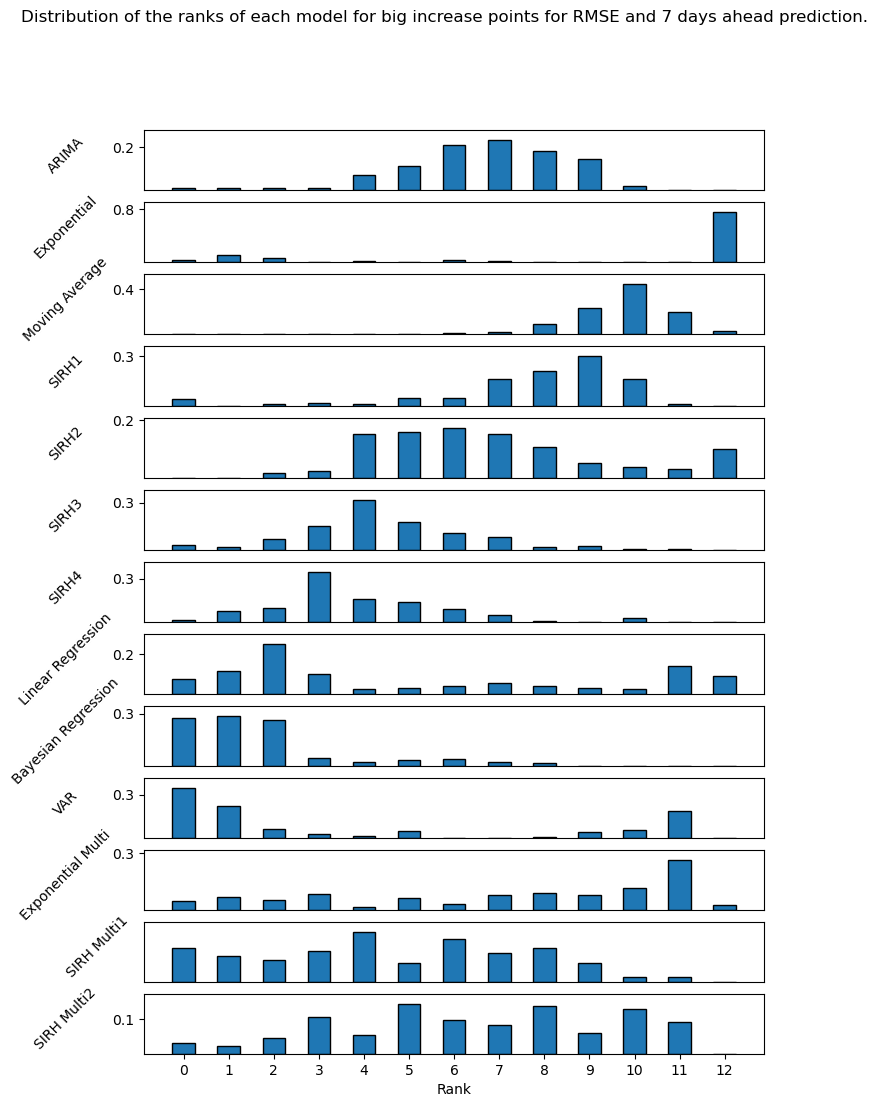
\includegraphics[width=0.7\textwidth]{figures/ranks_big_increase_RMSE_7.png}
    \caption{Distribution of rankings of the models for big increase points for 7-days ahead predictions and RMSE loss}
    \label{fig:rankings}
\end{figure}
This distribution of rankings of the model can be summed up in one single value : the expected value of the rank of a model (see \ref{fig:expected_rank} ), which enables to get the idea of the best model for this type of point, this loss, and this prediction range. 

\begin{figure}[h]
    \centering
    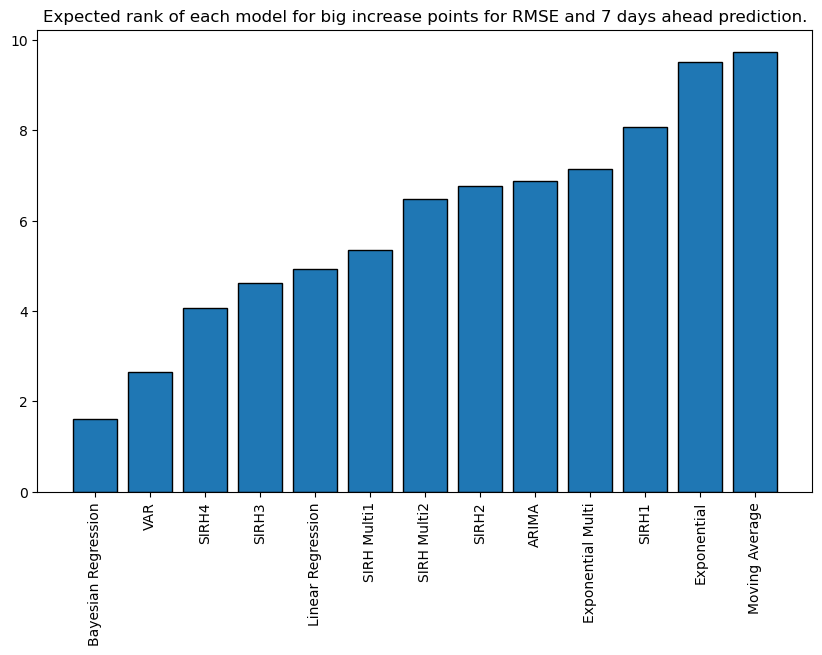
\includegraphics[width=0.7\textwidth]{figures/expected_ranks_big_increase_RMSE_7.png}
    \caption{Expected rank of the models for big increase points for 7-days ahead predictions and RMSE loss}
    \label{fig:expected_rank}
\end{figure}
This new number looses information (for instance on bimodal rankings distribution) but enables to enlight the expected performance of a model. 
For each loss and range of prediction, the expected rank of the models for each type of point can be vizualized on the same figure, which enables to have a global look of the performances of the models.(\ref{fig:heatmap_RMSE_7}) 
\begin{figure}[h]
    \centering
    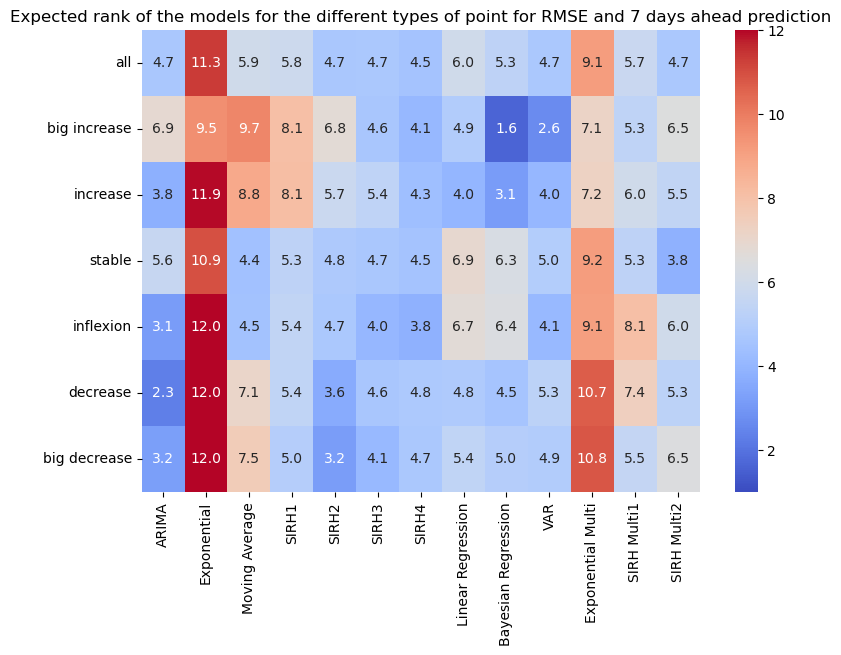
\includegraphics[width=0.7\textwidth]{figures/heatmap_RMSE_7.png}
    \caption{Expected rank of the models for each type of point for 7-days ahead predictions and RMSE loss}
    \label{fig:heatmap_RMSE_7}
\end{figure}


The other heatmaps corresponding to RMSE and WIS for 7 and 14 days ahead predictions can be found in the appendix (\ref{sec:appendix})
Some general interpretations can be made on these results. 
We noticed that regressors performances dropp from 7-days ahead to 14-days ahead. 
The family of the SIRH model does slightly better for long terms predictions than for short term ones. 
The ARIMA performance dropps from 7-days ahead to 14-days ahead predictions. 
The exponential models are very bad and almost always the last ones. 

\subsection{The Ensemble model}

It has been showned in the literature (TODO insert ref) that ensemble models, which are models taking into account the predictions of many individual models and output their mean, median, or any other function. 
We decided to implement or own ensemble models which are a linear combination of the predictions of the 13 individual models (without exponential models) for 7 and 14 days-ahead predictions.
The performances of these two models are showned in the two figure below (\ref{fig:esb_rank_7} and \ref{fig:esb_rank_14})

\begin{figure}
    \centering
    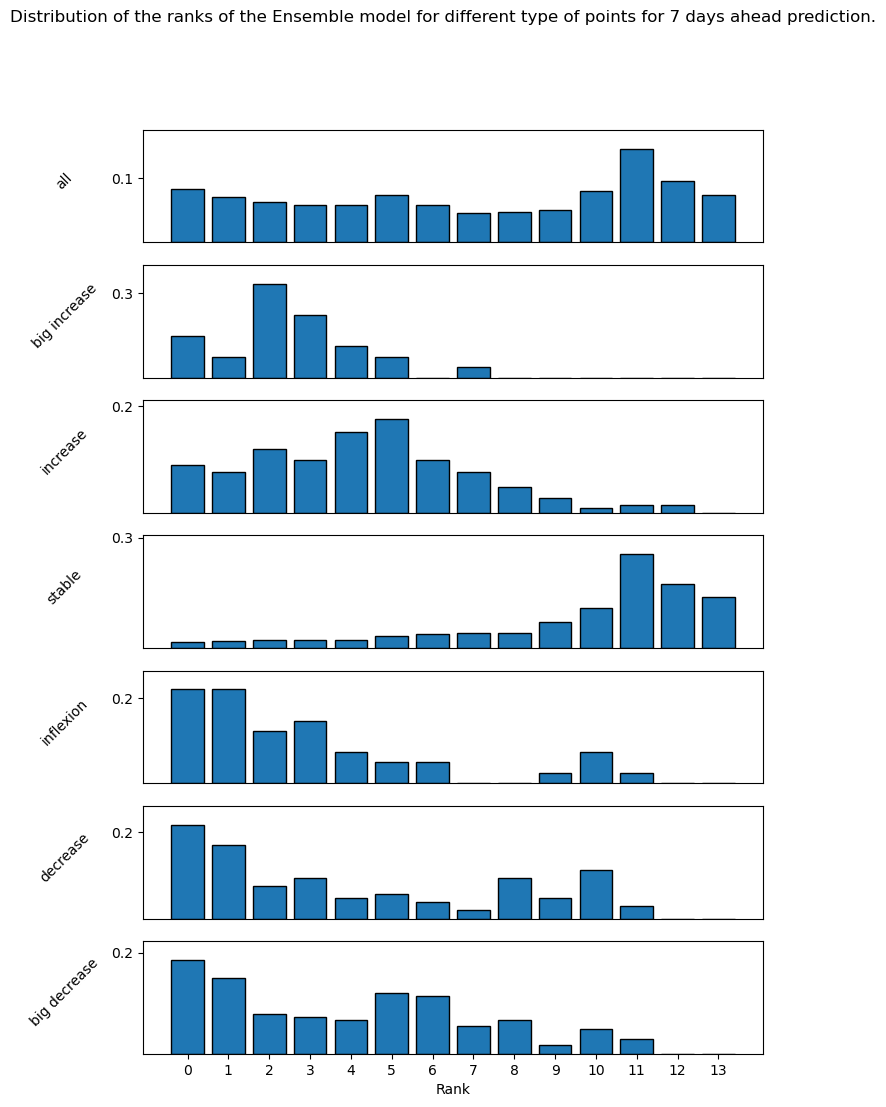
\includegraphics[width=0.7\textwidth]{figures/esb_rank_7.png}
    \caption{Expected rank of the ensemble model for each type of point for 7-days ahead predictions and RMSE loss}
    \label{fig:esb_rank_7}
\end{figure}

\begin{figure}
    \centering
    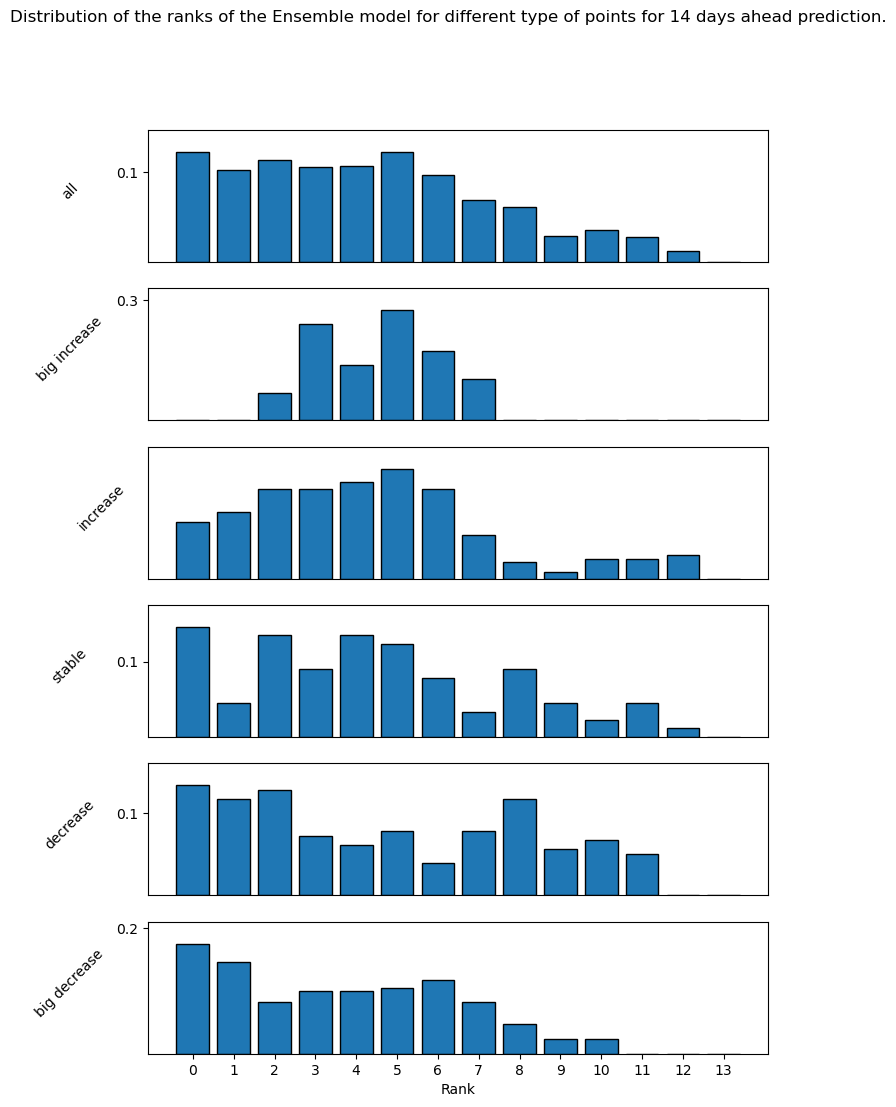
\includegraphics[width=0.7\textwidth]{figures/esb_rank_14.png}
    \caption{Expected rank of the ensemble model for each type of point for 14-days ahead predictions and RMSE loss}
    \label{fig:esb_rank_14}
\end{figure}

The distribution of the ranks of the ensemble model is almost always on the left side of the x-axis, except for the 'stable' points. 
The fact that the 'stable' points are overrepresented leads to a general poor performance of the ensemble model.
However, on the other type of points, the enesmble model is very consistent, and almpst always in the top models. 
the heatmaps of expected ranks help to see how consistent is the ensemble model (\ref{heatmap_esb_7} and \ref{heatmap_esb_14}). 

\begin{figure}
    \centering
    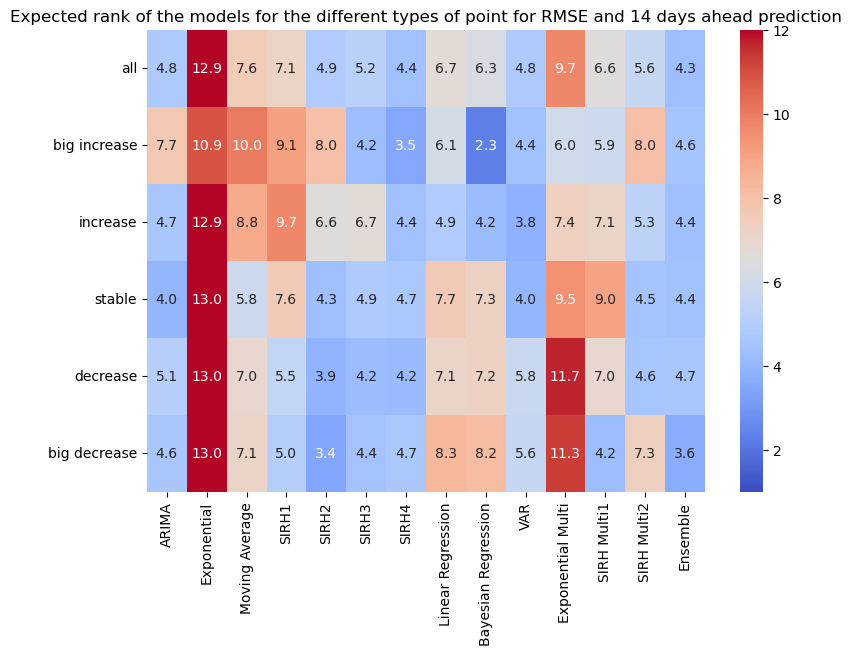
\includegraphics[width=0.7\textwidth]{figures/heatmap_esb_14.png}
    \caption{Expected rank of all the models for each type of point for 14-days ahead predictions and RMSE loss on the test set}
    \label{fig:heatmap_esb_14}
\end{figure}


\begin{figure}
    \centering
    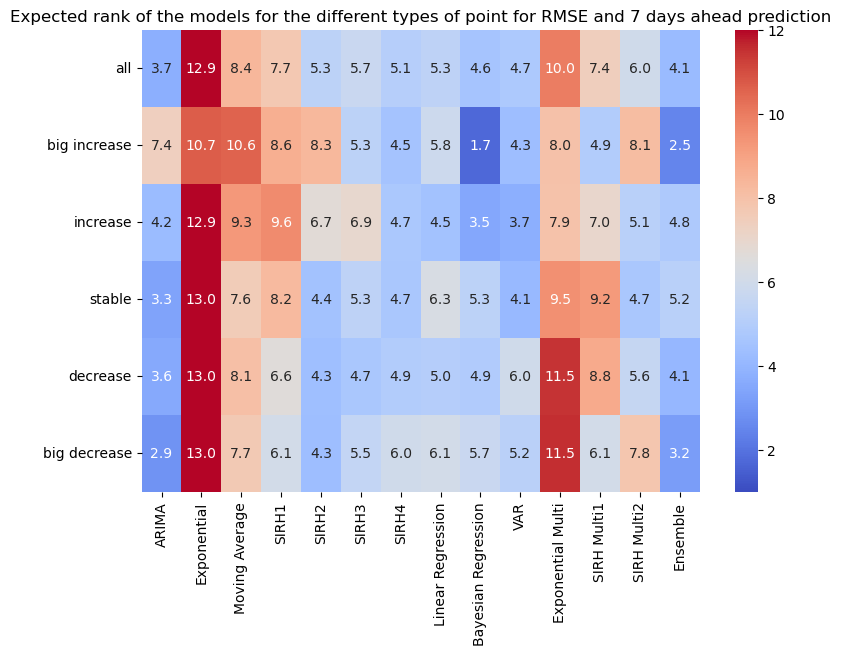
\includegraphics[width=0.7\textwidth]{figures/heatmap_esb_7.png}
    \caption{Expected rank of all the models for each type of point for 7-days ahead predictions and RMSE loss on the test set}
    \label{fig:heatmap_esb_7}
\end{figure}

From these figures, we can see that the ensemble model is rarely the best, but never the last model, as showed in TODO insert ref.
Its consticency enables to get good predictions and to avoid outliers predicted values.





